\section{Copyright Notice \& License}

    Copyright (C)  2024 Leandro Ebner. \\
    Permission is granted to copy, distribute and/or modify this document under the terms of the GNU Free Documentation License, Version 1.3 or any later version published by the Free Software Foundation; with no Invariant Sections, no Front-Cover Texts, and no Back-Cover Texts. A copy of the license can be found here:
    \href{https://www.gnu.org/licenses/fdl-1.3.txt}{https://www.gnu.org/licenses/fdl-1.3.txt}.

    \begin{figure}[h!]
    
\includegraphics{contents/figures/gfdl-logo.png}
    \end{figure}

    \vspace{5mm}
    

    This document is built using several packages originally developed by Stefan Gast for being compliant with RWU's corporate design. Due to fact that repository is archived now, an active fork is available for public at: \\
    \href{https://github.com/leandroebner/latex-rwustyle}{https://github.com/leandroebner/latex-rwustyle} 

    The source code to build this document, including all relevant information about the R2M project is available in a dedicated GitHub organization and actively maintained by it's contributors: \\
    \href{https://github.com/RWU-R2M}{https://github.com/RWU-R2M}

    
\section{Introduction}

    This document will serve as a comprehensive guide through the entire power distribution and wiring system of the rover. It meticulously details all relevant safety measures designed to minimize the likelihood of hazards or environmental damage. By following these guidelines, we aim to ensure that our work adheres to the highest safety standards. 

    \vspace{5mm}

    In addition to outlining essential safety protocols, this guide sets forth the minimum standards for both material and personal safety. These standards apply not only during the construction phase but also throughout the actual operation of all electronic components during the competition. To enhance understanding and clarity, it includes several schematics, data sheets, and detailed calculations. These resources are designed to provide a thorough illustration of the rover's internal architecture and functionality, making the document as informative and accessible as possible.

    \begin{table}[b!]
        \centering
        \begin{tabular}{|r|r|r|r|} \hline 
             Revision&  Date submitted& Summary of changes  &Authored \\ \hline 
             v1.0.0&  16.06.2024& Initial release  &Leandro Ebner \\ \hline
        \end{tabular}
    \end{table}

    \clearpage      
    
\section{Hazardous Material List}

    \subsection{Batteries}
    
    The rover is using two lithium-polymer based batteries (further referred to as LiPo batteries) to power all the electronics. Batteries, in general, are compliant with the regulations set by the CIRC (see \ref{battery} of the appendix) as long as they are sealed and follow certain safety guidelines. LiPo batteries are designed as permanently sealed units, which contain their electrolytes within durable casing materials. This prevents the escape of hazardous substances under normal operating conditions. This cell chemistry is widely used in consumer electronics, remote-controlled vehicles, and other devices where safety and environmental compliance are critical and high electrical characteristics are required. This demonstrates their reliability and safety under proper use and are known for a high energy density as well as output power capability. For this reason, the LiPo cell chemistry was also utilized for energy storage in the rover.
    
    \vspace{5mm}
    
    LiPo batteries feature a nominal voltage of around $3.7V$ per cell, depending on the exact type of internal chemistry. Higher output voltages are achieved by connecting several individual cells in series with each other, still being housed in the same battery enclosure. Therefore, the (series) cell count of a LiPo battery is a fundamental property of any LiPo battery and a direct measure for the expected output voltage. Usually, this property is indicated in the following way: "3S LiPo Battery", whereas "3S" is referring to a total series cell count of three. This results in a nominal voltage of around $11.1V$. For this exact reason, LiPo batteries can't be manufactured for an arbitrary output voltage and certain compromises must be made. The rover is built upon the idea of having a $24V$ battery supply as the main voltage for high power applications and another $12V$ battery supply for all logic and controlling components. This results in a 6S and 3S configuration of battery cells to closely match those voltages. Detailed information about the two batteries used in the rover can be found in their datasheet \ref{prim-battery} and \ref{sec-battery} respectively.

    \clearpage      
    
\section{Power Architecture}

    The rover's power architecture is divided into two separate power systems. This approach ensures galvanic isolation between the power and logic components, which is necessary to eliminate any possible wiring configuration in which a so-called "ground loop" could form. The underlying problem is based on the fact that there exists an interface and thus an electrical connection between the individual components. While the communication between power and logic components is implemented by establishing a physical connection between their corresponding GPIO pins and reading different voltage levels, there must be a precise reference voltage available at any given point in time. Generally speaking, this is done by using a common ground. Hence, the most basic form to utilize that common ground connection is to form a "star ground." If there are multiple paths to ground, a "ground loop" is present. These ground loops, in combination with wire inductance, can cause issues for high-current electronics like the rover's motor controllers (in this particular case utilizing ODrives). This is further illustrated in figure \ref{ground_loop_bad}.
    
    \begin{figure}[h]
    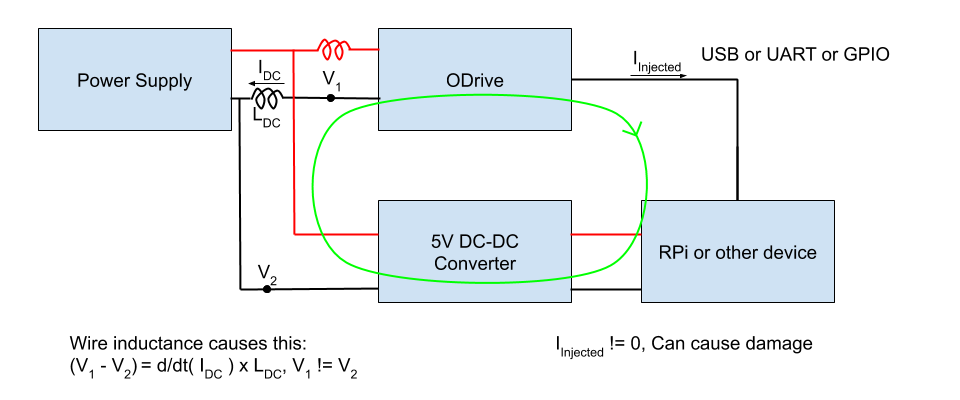
\includegraphics[width=\textwidth]{contents/figures/ground_loop_bad.png}
    \caption{Ground loop causes current flow $I_{Injected}$.}
    \label{ground_loop_bad}
    \end{figure}
    
    The issue is the inductance of the power wires between the motor controllers and the battery. This inductance, coupled with the high current drawn by the motor controllers, causes $V_1$ to be different as $V_2$, leading to potential mismatch in the voltage levels. As the motor controllers demand substantial current, the wire inductance can generate significant voltage drops along the power lines. If the voltage caused by the wire inductance and current is high enough, the 0-5V GPIO signals can swing much higher or lower than the defined voltage range, potentially exceeding safe operational limits. These fluctuations in voltage can introduce erratic behavior in the control system, compromising the performance and reliability of the motor controllers. This causes a current to flow through the ODrives GPIO pins, which can lead to unintended electrical noise and potential damage to sensitive electronic components.

    \clearpage
    \subsection{Reducing length of high-current wires}
    
    To mitigate these effects, it is substantial to keep the main powers as short as possible. All wires have some amount of inductance, which is an inherent property of any conductor through which current flows. The inductance is proportional to the length of the wires and the area of the loop formed by the power wires, meaning longer wires and larger loops will have higher inductance. This inductance can create unwanted resistance to changes in current flow, leading to voltage drops and potential interference with the system's performance. It is beneficial to keep those wires as short as possible and as close together as possible. By doing so, the loop area is minimized, and the inductance is reduced, thereby mitigating the adverse effects. However, this reduces the effect of the problem but does not eliminate it entirely, as even minimal inductance can cause issues in high-frequency and high-current applications.
    
    \subsection{Galvanic isolation}
    
    To completely minimize the possibility of creating ground loops by accident, the loop must be broken. This can be achieved by isolating the power supplies (no common ground) and connecting a dedicated signal ground between the logic and power electronics. An example of this is a single motor controller connected to a battery and a device like a Raspberry Pi connected to a different battery. It is possible to achieve the same functionality with a DC/DC isolator as shown in figure \ref{ground_loop_fix}. By isolating the data connection (whether it is GPIO, USB, or UART, etc.), the ground loop is broken.
    
    \begin{figure}[h]
    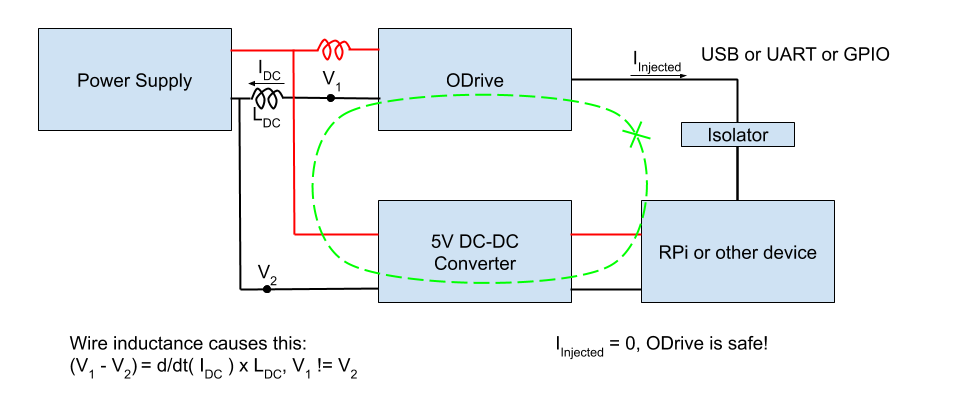
\includegraphics[width=\textwidth]{contents/figures/ground_loop_fix.png}
    \caption{Mismatched voltage levels wont introduce unwanted current flows.}
    \label{ground_loop_fix}
    \end{figure}

    \clearpage
    \subsection{Basic Electric Layout}

    The main energy storage contains two unregulated $24V$ (6S) and $12V$ (3S) power sources in the form of LiPo batteries. This part of the rover also integrates a dedicated battery management system (further referred to as BMS) for each battery. Additionally, the main fusing for the primary \& secondary battery can be found. The fuses protect the rover's circuitry as well as the batteries themselves. Due to the fact, that these components are strictly connected to the individual batteries, they change frequently with each battery exchange during normal operation. This means that during missions, the batteries can be quickly replaced without affecting other parts of the rover. Therefore, this area is separated from other areas of the rover's wiring as it is the only region where connections and disconnections of components are allowed. This separation is crucial to avoid accidental disconnections that could affect the rover's operation or create potential risks by introducing faulty connections. The output of both batteries is directly fed into an emergency stop system. Afterwards, the power travels into two separate distribution and fusing circuits before supplying the actual components and voltage converters further down the line.
    
    \begin{figure}[h]
    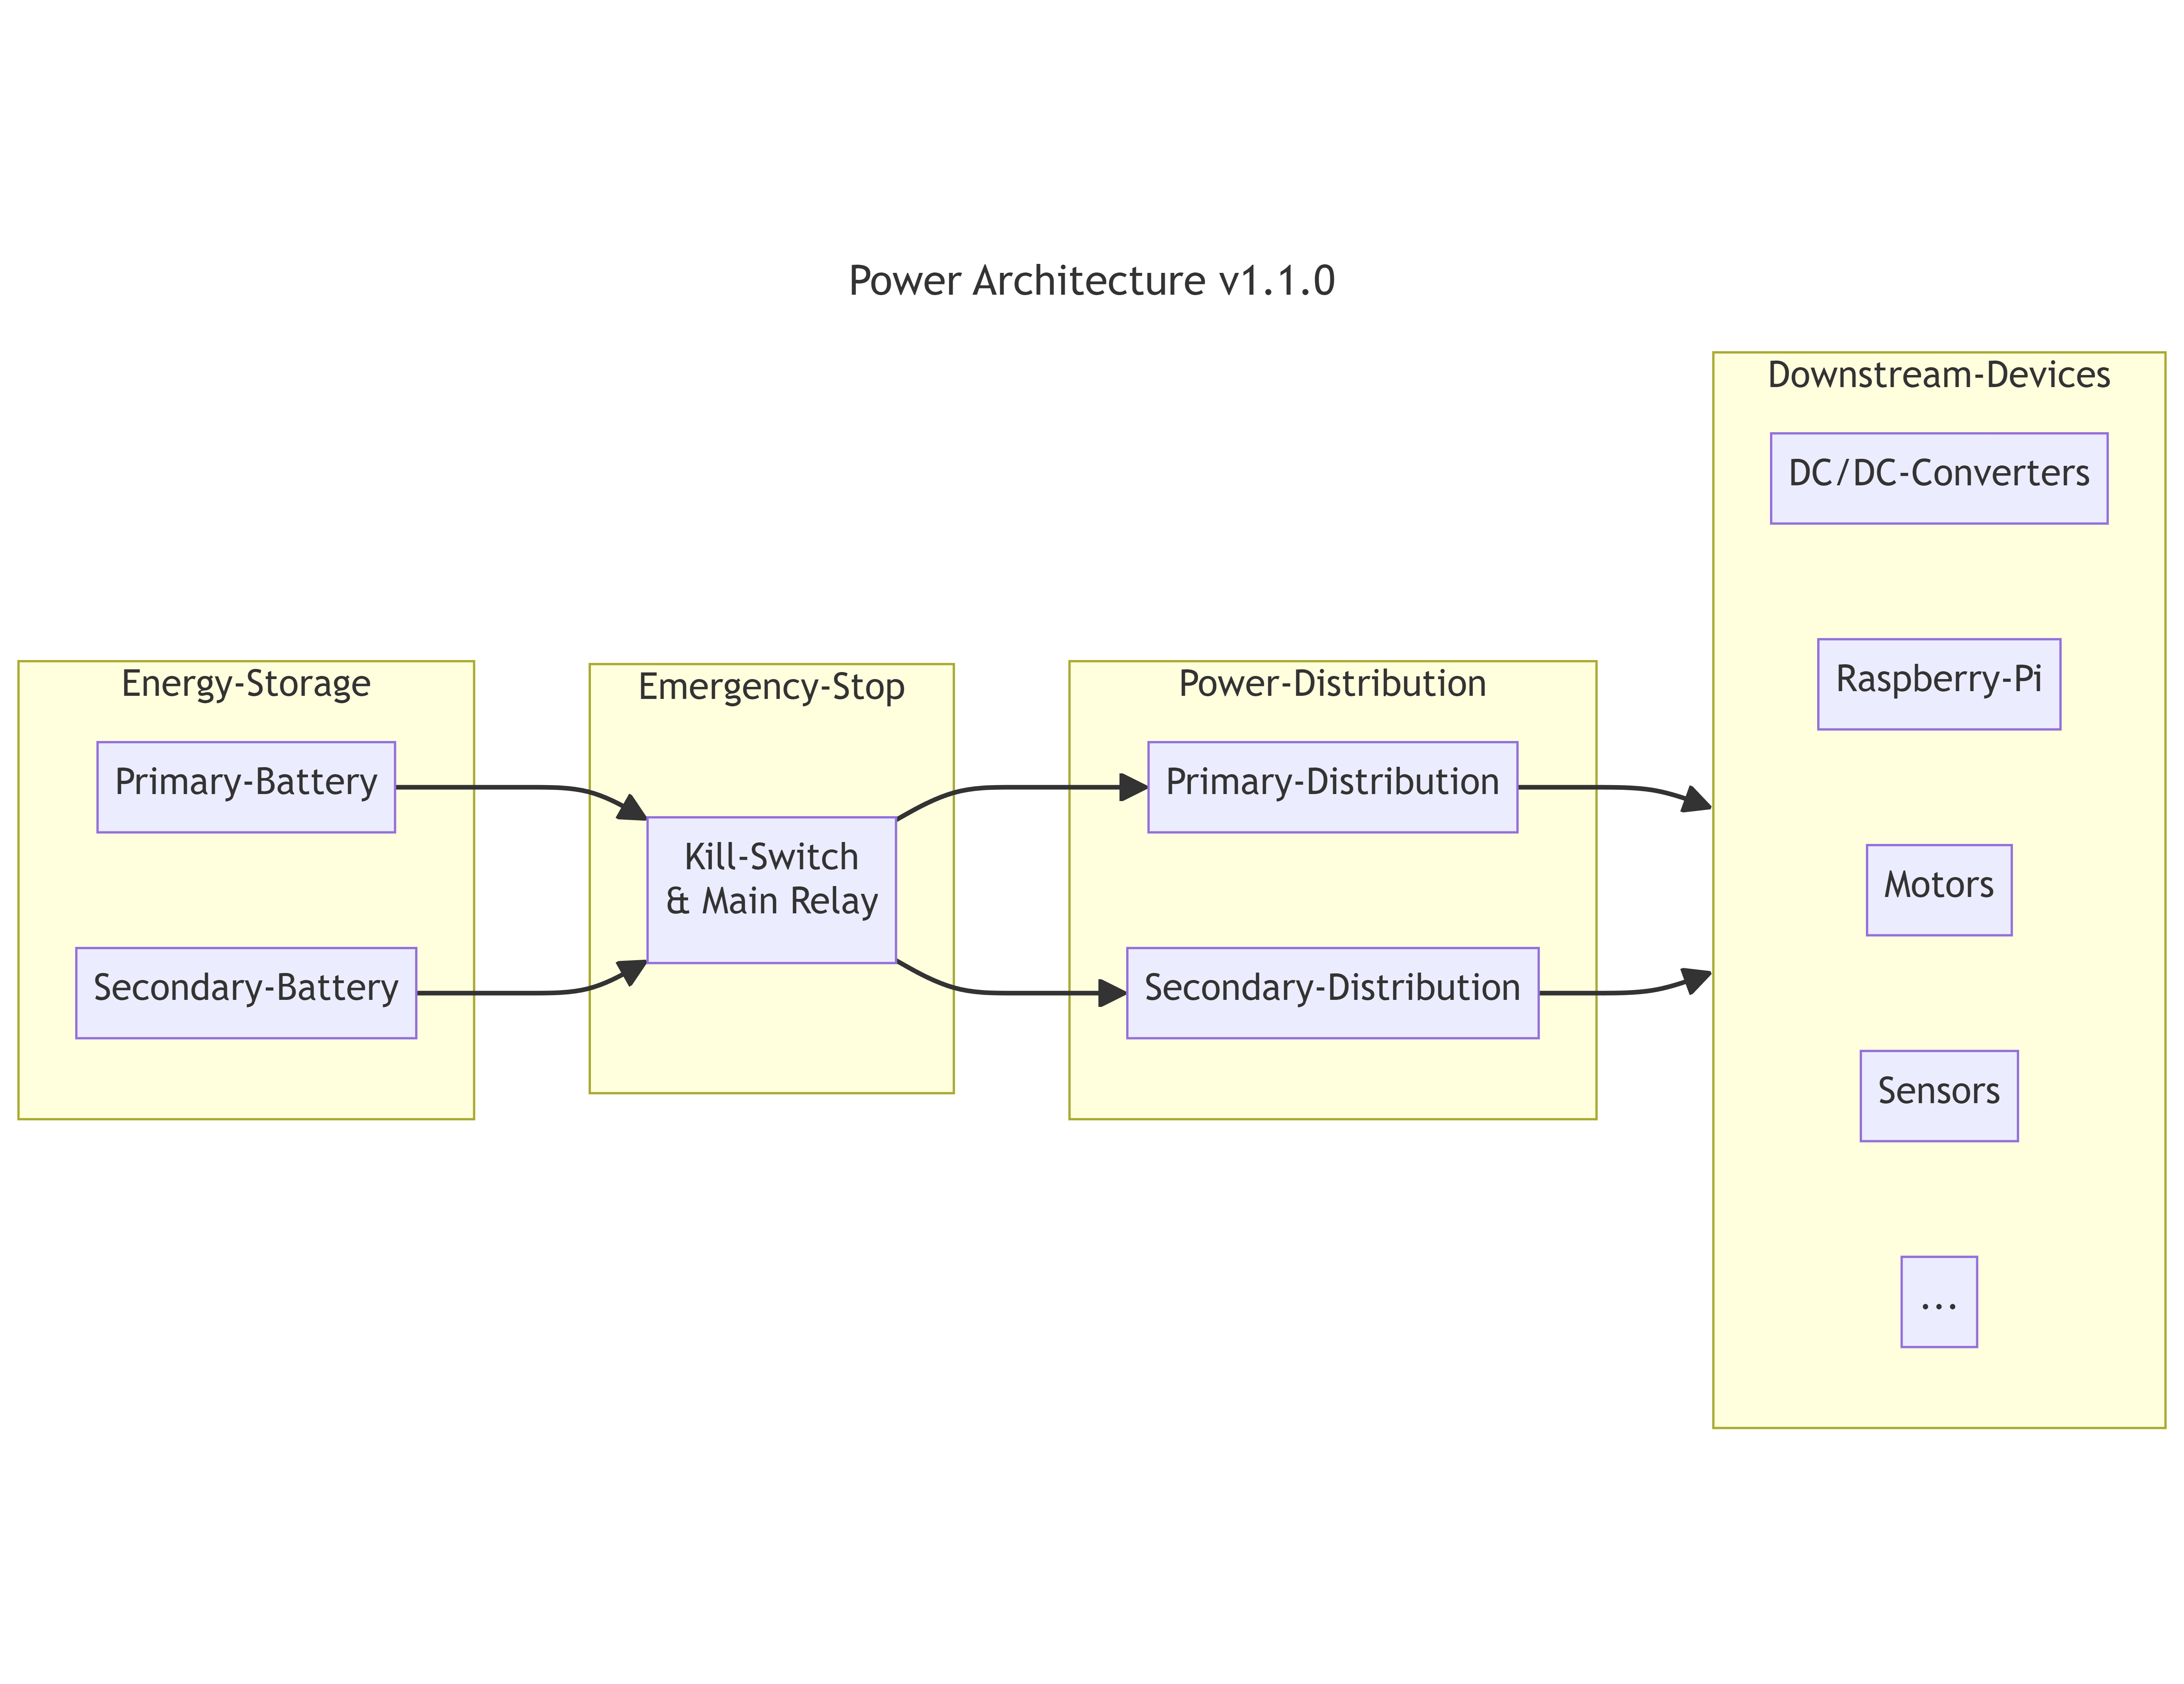
\includegraphics[width=\textwidth]{contents/figures/power-architecture-v1.1.0.png}
    \caption{Basic electrical layout split in the main 4 categories. Each category serves a different purpose (i.e. safely distributing the power or connecting the individual components).}
    \label{power_architecture}
    \end{figure}

    \clearpage

    

    
    \begin{table}
        \centering
        \begin{tabular}{|r|r|r|r|r|} \hline 
             color&  code &  cross-section&  equivalent to& ampacity\\ \hline 
             white&  WH \#FFFFFF&  $0,5mm^2$&  21 AWG& 7 Amps\\ \hline 
             black&  BK \#000000&  $1,5mm^2$&  16 AWG& 18 Amps\\ \hline 
             grey&   GY \#808080&  $4,0mm^2$&  12 AWG& 30 Amps\\ \hline 
             red&    RD \#FF0000&  $10,0mm^2$&  8 AWG& 55 Amps\\ \hline
        \end{tabular}
        \caption{Caption}
        \label{color-codes}
    \end{table}

    \clearpage

    \begin{figure}[h!]
    \centering
    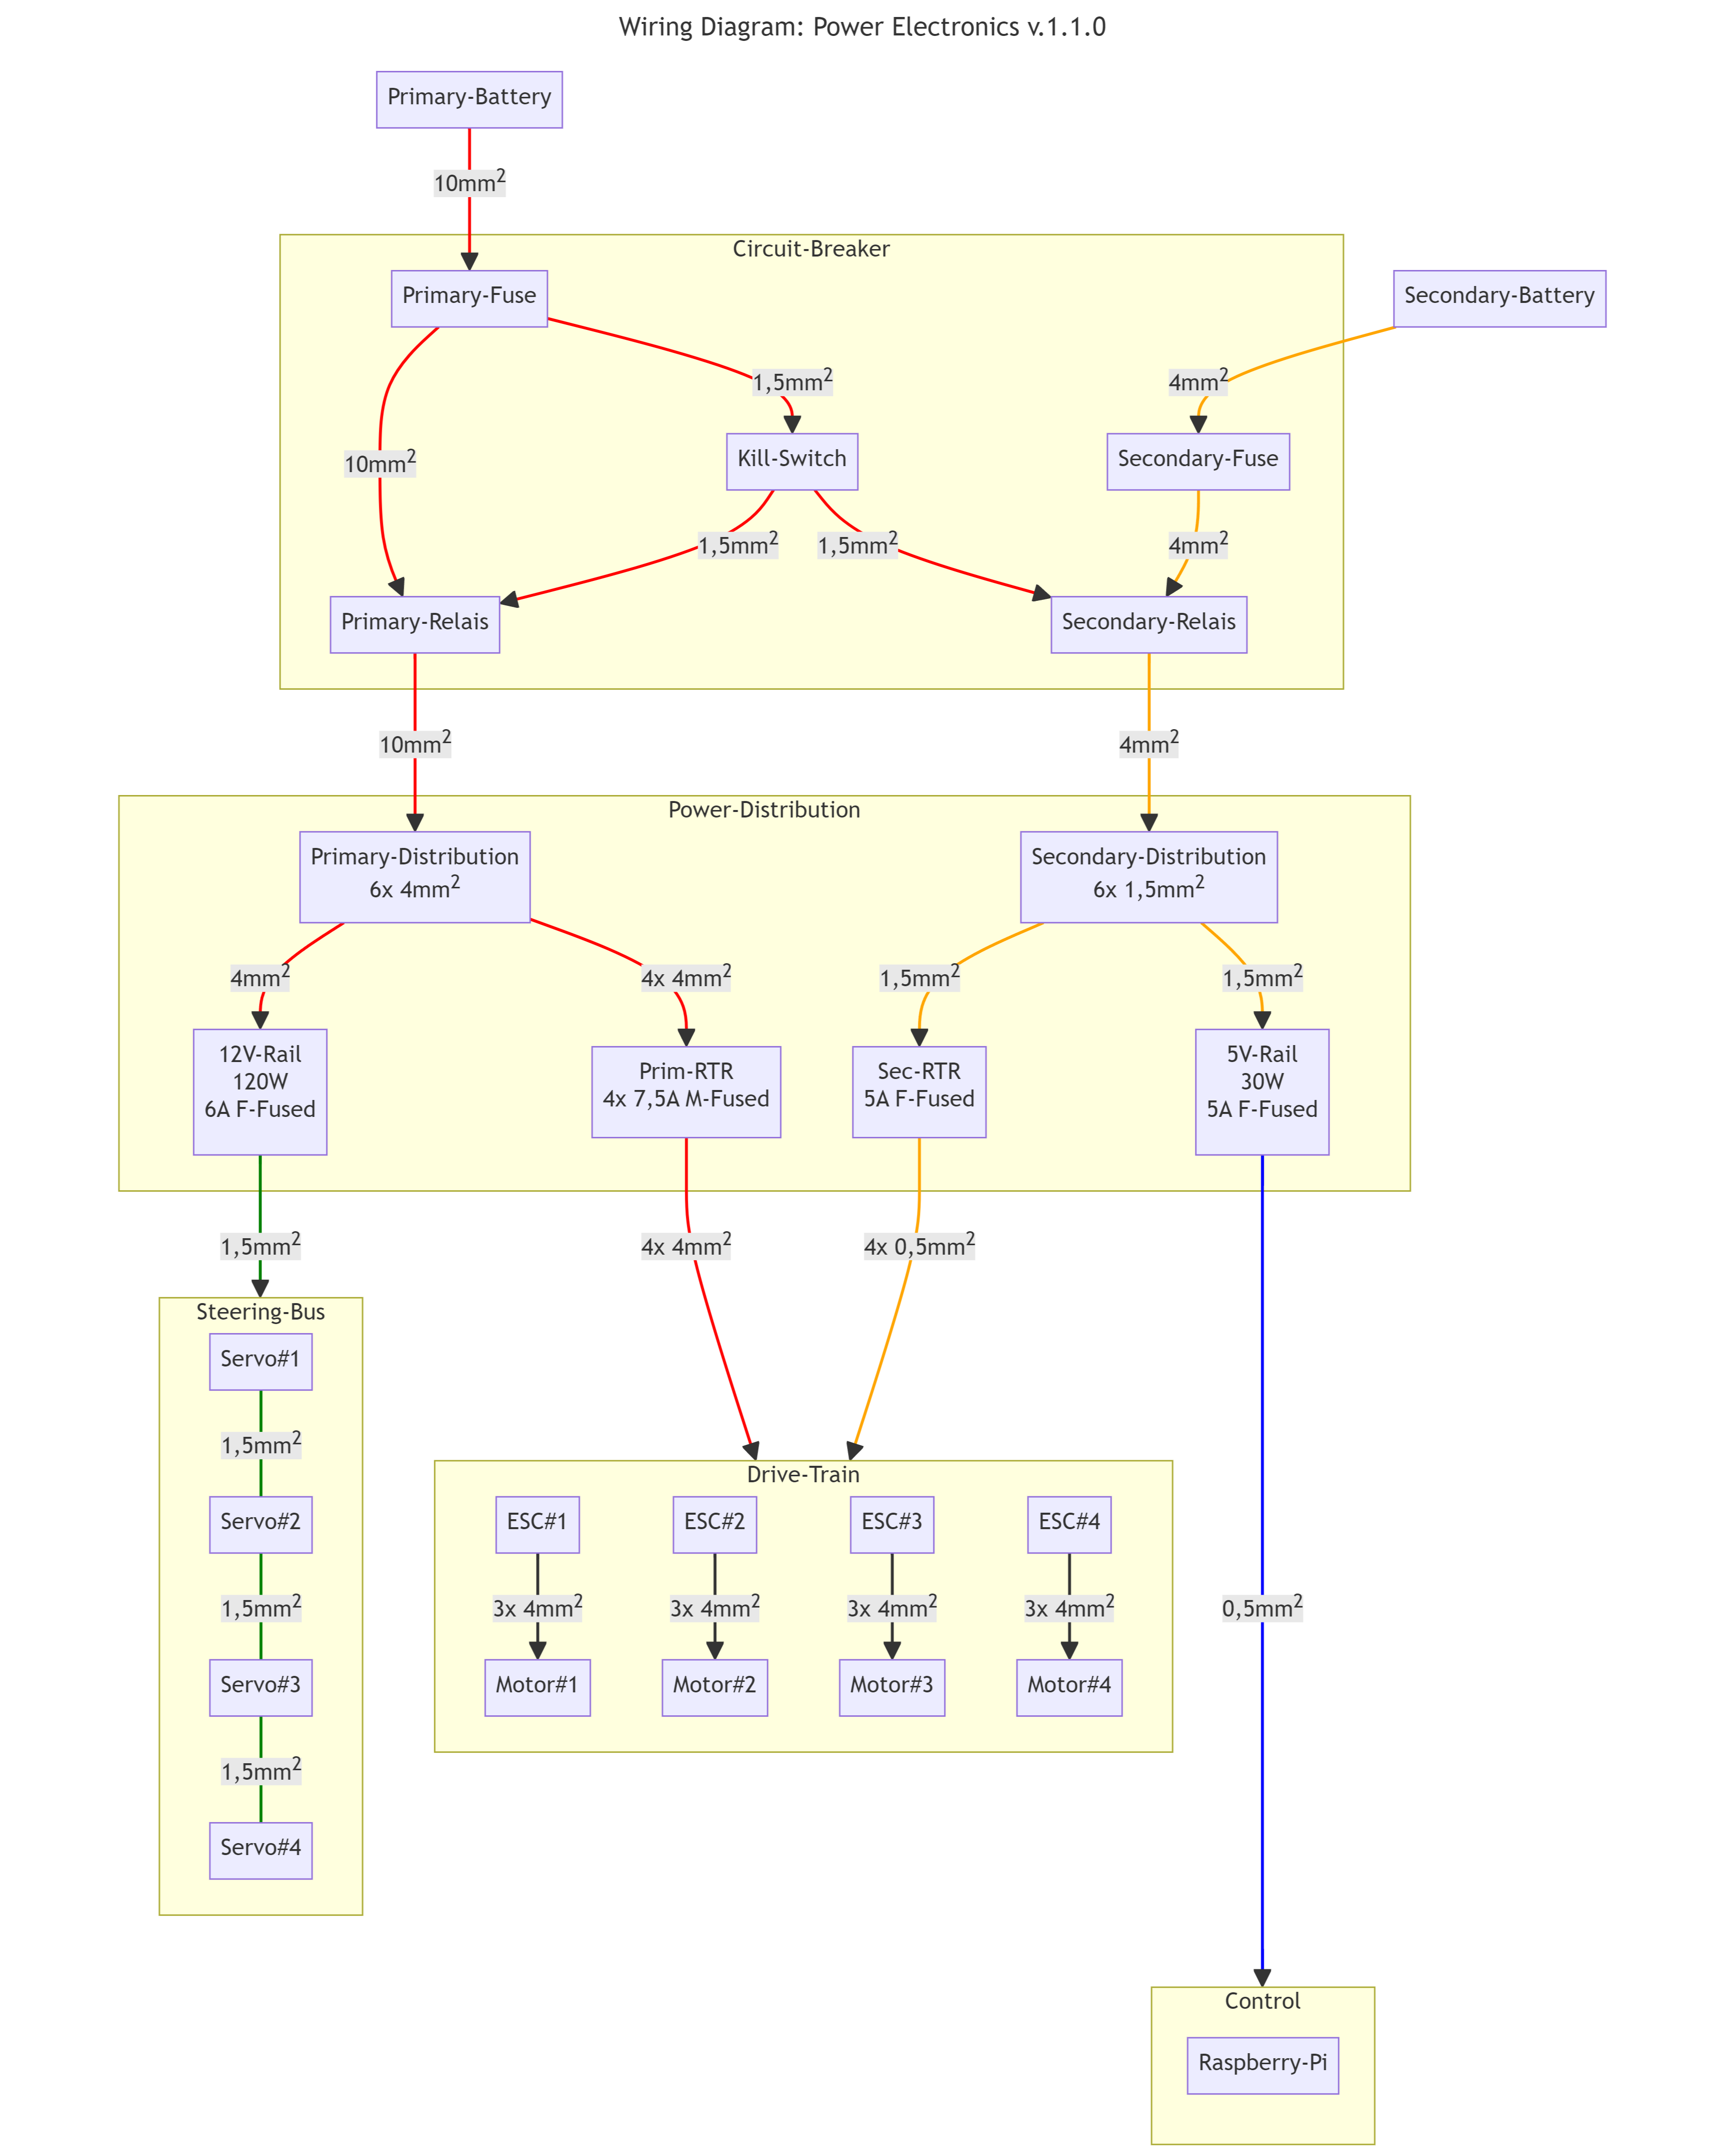
\includegraphics[width=1\textwidth]{contents/figures/wiring-diagram-p-v1.1.0.png}
    \caption{tst}
    \label{wiring_power}
    \end{figure}

    




\section{Energy Storage}

\section{Emergency Stop}

\section{Power Distribution}

\section{Power Conversion}

\section{Power Consuming Circuits}

\section{Unused Circuits}

\section{Circuit Table}

\section{Appendix}

    \subsection{Definitions}

    \begin{enumerate}
        \item The word \textit{should} indicates a suggestion which may become a requirement in future competitions.
        \item A \textit{circuit} is one or more electricity-consuming devices (and the connections between them) which draw current from a single power source through a common \textit{circuit protection} element.
        \item \textit{Regulators} consume and provide power, with their input and outputs counting as at least one \textit{circuit} each.
        \item The \textit{current rating} of a component is the manufacturer-published value indicating the maximum acceptable amperage consumed or provided by the device in normal continuous conditions. Transient, burst, or peak current limits are \textbf{not} current ratings.
        \item The \textit{current rating} of \textit{circuit protection} is the amperage above which it is designed to interrupt current flow.
        \item \textit{Circuit protection} is a fuse or electromechanical circuit-breaker which reliably interrupts excessive current flows through a connected \textit{circuit}. Software-based solutions are \textbf{insufficient}. Motor controllers, power regulators, or other devices with current limiting capabilities are \textbf{not} sufficient for use as circuit protection. Self-resetting fuses are also \textbf{insufficient}.
        \item A \textit{kill switch} is a physical switch mounted on a rover which, when pressed down, causes the interruption of power to \textbf{all} rover systems until the switch is manually reset.
    \end{enumerate}

    \clearpage

    \subsection{Safety Requirements}
    


    \begin{enumerate}
        %---------------------------------------------------------------------------------------------------------------------------------------------------------------------------------------
        \item The rover must not include any flammable, environmentally damaging, or otherwise hazardous liquids or gasses, except:
        \begin{enumerate}
            \item Within a permanently sealed component such as a battery; \label{battery}
            \item Commercially-available lubricants as required by mechanical assemblies, where care is taken to avoid overuse and contamination. \label{lubricants}
        \end{enumerate}
        %---------------------------------------------------------------------------------------------------------------------------------------------------------------------------------------
        \item Each rover must be equipped with at least one kill switch:
        \begin{enumerate}
            \item The pressable area of the kill switch must be at least $10cm^2$ and red in color. Levers or toggle switches are not acceptable.
            \item No other button on the rover may be red.
            \item Kill switches must be mounted on the top of the rover, with the button oriented toward the sky in the rover’s normal driving orientation.
            \item A keep out region must be maintained around the kill switch with a radius of $15cm$: No components taller than the base of the kill switch may intrude on the keep out region.
            \item Kill switches must not be obstructed by a cover or sleeve which extends above the pressable surface, and must be mounted such that it will not be obstructed by other components during rover operation.
            \item The circuit including the kill switch must include appropriate circuit protection, and the “break” or “disconnect” current rating of the kill switch must exceed the current rating of the circuit protection.
            \item The function of the kill switch must not depend on the integrity of any power source or computerized system. Indirect switching by relays or similar devices is permitted as long as these are driven by the kill switch, and reliably turn off when their control line is disconnected.
            \item The function of the kill switch must not depend on the integrity of any particular wiring connection; for example, physically tearing the kill switch off the rover should produce the same effect as pressing it.
            \item If multiple kill switches are installed on the rover, pressing any one must cut all power to to the rover.
            \item The function of the kill switch must not be disabled or bypassed by any means.
            \item Rovers should have a remote motion stop for disabling a run-away rover, such as a dead man’s switch on a lead, or a radio-frequency system that operates independently of the rover communications system.
        \end{enumerate}
        %---------------------------------------------------------------------------------------------------------------------------------------------------------------------------------------

    \clearpage

        %---------------------------------------------------------------------------------------------------------------------------------------------------------------------------------------
        \item Each battery must include or be installed with a single circuit protection element which protects all circuits supplied by the battery, and the battery itself.
        \begin{enumerate}
            \item The current rating of this protection must not exceed the lesser of:
            \begin{enumerate}
                \item The current rating of the battery;
                \item 150\% of the sum of the current ratings of all connected circuits.
            \end{enumerate}
            \item This circuit protection must be installed as close as possible to the battery.
            \item Each battery must be protected by a battery management system that provides under-voltage lockout protection.
            \begin{enumerate}
                \item The battery management system should provide cell voltage monitoring, over-current protection, and over-voltage protection.
                \item Batteries should be connected to their battery management systems at all times, not only when installed on the rover.
            \end{enumerate}
            \item All wiring and connecting hardware between the battery and circuit protection must be fully secured and insulated such that no reasonable impact, vibration, loose object, or liquid could possibly create an unprotected short circuit.
            \item If multiple batteries are used, each must have its own fuse according to these requirements. You may not connect multiple batteries without a circuit protection element per battery.
            \item Multiple batteries may only be connected in series only if they feed a single circuit and each battery has a battery management system with under-voltage-lockout.
            \item Teams are responsible for the proper disposal of any compromised electrical components and/or batteries.
            \item Teams should store batteries in fireproof bags (ie Lipo storage bag).
        \end{enumerate}
        %---------------------------------------------------------------------------------------------------------------------------------------------------------------------------------------
        \item 
    \end{enumerate}




